\documentclass{beamer}
\usepackage{amsmath}
\usepackage{hyperref}
\usepackage{listings}
\usepackage{xcolor}
\hypersetup{colorlinks=true, citecolor=blue, filecolor=blue, linkcolor=blue, urlcolor=blue}
\definecolor{codegreen}{rgb}{0,0.6,0}
\definecolor{codegray}{rgb}{0.5,0.5,0.5}
\definecolor{codepurple}{rgb}{0.58,0,0.82}
\definecolor{backcolour}{rgb}{0.95,0.95,0.92}
 
\lstdefinestyle{mystyle}{
    backgroundcolor=\color{backcolour},   
    commentstyle=\color{codegreen},
    keywordstyle=\color{magenta},
    numberstyle=\tiny\color{codegray},
    stringstyle=\color{codepurple},
    basicstyle=\ttfamily\footnotesize,
    breakatwhitespace=false,         
    breaklines=true,                 
    captionpos=b,                    
    keepspaces=true,                 
    %numbers=left,                    
    numbersep=5pt,                  
    showspaces=false,                
    showstringspaces=false,
    showtabs=false,                  
    tabsize=2
}
 
\lstset{style=mystyle}

\mode<presentation> {

% The Beamer class comes with a number of default slide themes
% which change the colors and layouts of slides. Below this is a list
% of all the themes, uncomment each in turn to see what they look like.

%\usetheme{default}
\usetheme{AnnArbor}
%\usetheme{Antibes}
%\usetheme{Bergen}
%\usetheme{Berkeley}
%\usetheme{Berlin}
%\usetheme{Boadilla}
%\usetheme{CambridgeUS}
%\usetheme{Copenhagen}
%\usetheme{Darmstadt}
%\usetheme{Dresden}
%\usetheme{Frankfurt}
%\usetheme{Goettingen}
%\usetheme{Hannover}
%\usetheme{Ilmenau}
%\usetheme{JuanLesPins}
%\usetheme{Luebeck}
%\usetheme{Madrid}
%\usetheme{Malmoe}
%\usetheme{Marburg}
%\usetheme{Montpellier}
%\usetheme{PaloAlto}
%\usetheme{Pittsburgh}
%\usetheme{Rochester}
%\usetheme{Singapore}
%\usetheme{Szeged}
%\usetheme{Warsaw}

% As well as themes, the Beamer class has a number of color themes
% for any slide theme. Uncomment each of these in turn to see how it
% changes the colors of your current slide theme.

%\usecolortheme{albatross}
%\usecolortheme{beaver}
%\usecolortheme{beetle}
%\usecolortheme{crane}
%\usecolortheme{dolphin}
%\usecolortheme{dove}
%\usecolortheme{fly}
%\usecolortheme{lily}
%\usecolortheme{orchid}
%\usecolortheme{rose}
%\usecolortheme{seagull}
%\usecolortheme{seahorse}
%\usecolortheme{whale}
%\usecolortheme{wolverine}

%\setbeamertemplate{footline} % To remove the footer line in all slides uncomment this line
\setbeamertemplate{footline}[page number] % To replace the footer line in all slides with a simple slide count uncomment this line

\setbeamertemplate{navigation symbols}{} % To remove the navigation symbols from the bottom of all slides uncomment this line
}

\usepackage{graphicx} % Allows including images
\usepackage{booktabs} % Allows the use of \toprule, \midrule and \bottomrule in tables
%\usepackage {tikz}
\usepackage{tkz-graph}
\GraphInit[vstyle = Shade]
\tikzset{
  LabelStyle/.style = { rectangle, rounded corners, draw,
                        minimum width = 2em, fill = yellow!50,
                        text = red, font = \bfseries },
  VertexStyle/.append style = { inner sep=5pt,
                                font = \normalsize\bfseries},
  EdgeStyle/.append style = {->, bend left} }
\usetikzlibrary {positioning}
%\usepackage {xcolor}
\definecolor {processblue}{cmyk}{0.96,0,0,0}
%----------------------------------------------------------------------------------------
%	TITLE PAGE
%----------------------------------------------------------------------------------------

\title[Optimization]{Numerical Optimization 01: Introduction} % The short title appears at the bottom of every slide, the full title is only on the title page

\author{Qiang Zhu} % Your name
\institute[University of Nevada Las Vegas] % Your institution as it will appear on the bottom of every slide, may be shorthand to save space
{
University of Nevada Las Vegas\\ % Your institution for the title page
\medskip
}
\date{\today} % Date, can be changed to a custom date

\begin{document}

\begin{frame}
\titlepage % Print the title page as the first slide
\end{frame}

\begin{frame}
\frametitle{Overview} % Table of contents slide, comment this block out to remove it
\tableofcontents % Throughout your presentation, if you choose to use \section{} and \subsection{} commands, these will automatically be printed on this slide as an overview of your presentation
\end{frame}

%----------------------------------------------------------------------------------------
%	PRESENTATION SLIDES
%----------------------------------------------------------------------------------------

%------------------------------------------------

\section{Syllabus}
\begin{frame}{Syllabus}

    
\begin{columns}

\begin{column}{.6\textwidth}
We have two goals: 
\begin{itemize}
    \item Learn Julia programming
    \item Understand the optimization methods
\end{itemize}
Subjects to be covered
\begin{itemize}
    \item Julia programming
    \item Local Optimization
    \begin{itemize}
        \item Derivatives and Gradients
        \item Bracketing
        \item First/second-Order optimization
        \item Gradient free methods
        \item Stochastic methods
    \end{itemize}
    \item Global Optimization
    \item Sampling Plans
    \item Surrogate Optimization
    \item Expression Optimization

\end{itemize}
\end{column}
\begin{column}{.4\textwidth}
\begin{figure}
\centering

\includegraphics[width=30mm]{Figs/algo_opt.jpg}
\end{figure}
Virtual Meet twice a week (~90 minutes each time).\\
\begin{itemize}
    \item review of homework (20-30 mins)
    \item lecture (30-50 mins)
    \item coding (20-30 mins)
\end{itemize}
\end{column}

\end{columns}

\end{frame}

\section{Why Optimization?}
\begin{frame}{Why optimization}
\begin{columns}
\begin{column}{.55\textwidth}
A typical optimization problem is to 
\begin{equation*}
\begin{split}
    \textrm{minimize} &~~ f(x)\\
    \textrm{subject to} &~~ x \in X    
\end{split}
\end{equation*}
A design point ($x$) can be represented as a vector of values
corresponding to different design variables.
\end{column}

\begin{column}{.45\textwidth}
\begin{figure}
\centering
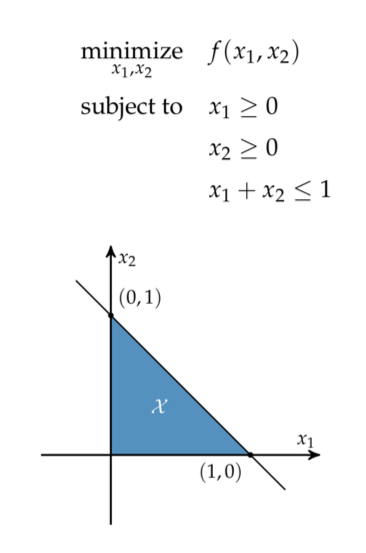
\includegraphics[width=40mm]{Figs/solution-space.jpeg}
\end{figure}
\end{column}
\end{columns}

A \textcolor{blue}{necessary condition?} for $f(x)$ reaches the minimum is that \textcolor{blue}{$f`(x)=0$}.
\end{frame}


\begin{frame}{Optimization is hard!}
\begin{itemize}
    \item $f`(x)=0$ is not a sufficient condition.
\begin{figure}
\centering
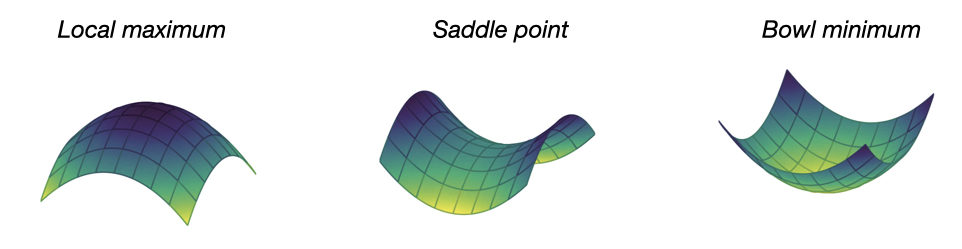
\includegraphics[width=80mm]{Figs/minimum.jpeg}
\end{figure}
    \item There exist many points where {$f`(x)=0$}.
\begin{figure}
\centering
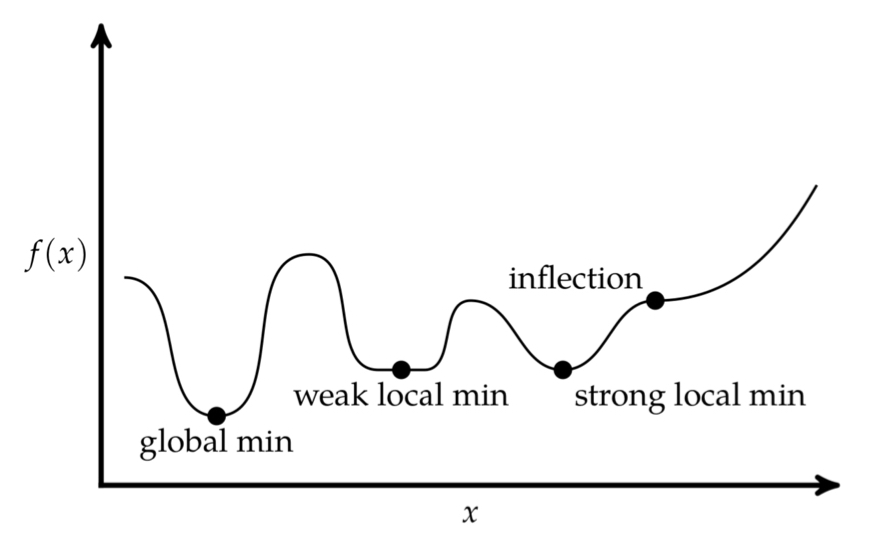
\includegraphics[width=60mm]{Figs/multi-minima.jpeg}
\end{figure}
    \item $f(x)$ and $f`(x)$ are hard to evaluate.

\end{itemize}
\end{frame}


\section{Why Julia?}
\begin{frame}{Why Julia?}
\textcolor{red}{Run Julia at } \url{https://www.juliabox.com}

\begin{columns}

\begin{column}{.5\textwidth}
\begin{itemize}
    \item Math-friendly
    \item Looks like Python 
    \item Runs like C/Fortran
    \item Growing ecosystem
\end{itemize}
\end{column}

\begin{column}{.5\textwidth}
\begin{figure}
\centering

\includegraphics[width=40mm]{Figs/julia.png}
\end{figure}
\end{column}
\end{columns}
\begin{figure}
\centering
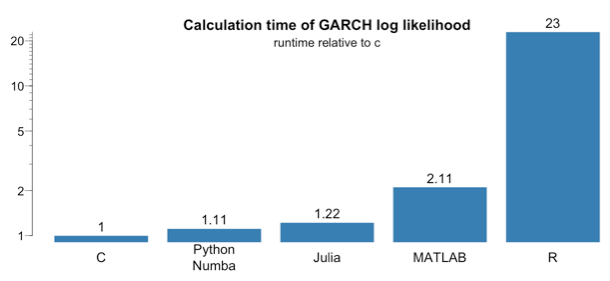
\includegraphics[width=90mm]{Figs/julia-comp.png}
\end{figure}
\end{frame}


\section{Summary}
\begin{frame}{Summary}
    \begin{itemize}
        \item Optimization in engineering is the process of finding the best system design subject to a set of constraints.
        \item Optimization can be transformed to a math problem but it is sometimes hard to solve
        \item We will extensively using the Julia language to learn how to solve the optimization numerically
    \end{itemize}
\end{frame}


\section{Homework}
\begin{frame}{Homework}
In Julia, write the following trial functions, make the contour plots and analyze their minima behavior.
\begin{itemize}
    \item Booth's function
    \begin{equation*}
        f(x_1, x_2) = (x_1 + 2x_2 -7)^2 + (2x_1 + x_2 -5)^2
    \end{equation*}

    \item Barnin function
    \begin{equation*}
        f(x_1, x_2) = a(x_2 - bx_1^2 + cx_1 - r)^2 + s(1-t)cos(x_1) +s
    \end{equation*}
    where $a=1, b=5.1/(4\pi^2), c=5/\pi, r=6, s=10, t=1/8\pi$.
    
    \item Rosenbrock's Banana function
    \begin{equation*}
        f(x_1, x_2) = (a-x_1)^2 + b(x_2-x_1^2)^2
    \end{equation*}
    where $a=1, b=5$.
    
\end{itemize}
More functions can be found at \url{https://en.wikipedia.org/wiki/Test_functions_for_optimization}
\end{frame}

\end{document}

